\documentclass{ximera}

\newcommand{\dfn}{\textbf}
\renewcommand{\vec}[1]{{\overset{\boldsymbol{\rightharpoonup}}{\mathbf{#1}}}\hspace{0in}}
%% Simple horiz vectors
\renewcommand{\vector}[1]{\left\langle #1\right\rangle}
\newcommand{\arrowvec}[1]{{\overset{\rightharpoonup}{#1}}}
\newcommand{\R}{\mathbb{R}}
\newcommand{\transpose}{\intercal}
\newcommand{\ro}{\texttt{R}}%% row operation
\newcommand{\dotp}{\bullet}%% dot product

\usetikzlibrary{calc,bending}
\tikzset{>=stealth}


\usepackage{mdframed} % For framing content
%\usepackage{ifthen}   % For conditional statements

% Define the 'concept' environment with an optional header
\newenvironment{concept}[1][]{%
  \begin{mdframed}[linecolor=black, linewidth=2pt, innertopmargin=5pt, innerbottommargin=5pt, skipabove=12pt, skipbelow=12pt]%
    \noindent\large\textbf{#1}\normalsize%
}{%
  \end{mdframed}%
}











%% \colorlet{textColor}{black}
%% \colorlet{background}{white}
%% \colorlet{penColor}{blue!50!black} % Color of a curve in a plot
%% \colorlet{penColor2}{red!50!black}% Color of a curve in a plot
%% \colorlet{penColor3}{red!50!blue} % Color of a curve in a plot
%% \colorlet{penColor4}{green!50!black} % Color of a curve in a plot
%% \colorlet{penColor5}{orange!80!black} % Color of a curve in a plot
%% \colorlet{penColor6}{yellow!70!black} % Color of a curve in a plot
%% \colorlet{fill1}{penColor!20} % Color of fill in a plot
%% \colorlet{fill2}{penColor2!20} % Color of fill in a plot
%% \colorlet{fillp}{fill1} % Color of positive area
%% \colorlet{filln}{penColor2!20} % Color of negative area
%% \colorlet{fill3}{penColor3!20} % Fill
%% \colorlet{fill4}{penColor4!20} % Fill
%% \colorlet{fill5}{penColor5!20} % Fill
%% \colorlet{gridColor}{gray!50} % Color of grid in a plot


\author{Bart Snapp}

\title{Vector spaces}

\begin{document}
\begin{abstract}
  We describe properties of vectors and matrices and discuss their
  implications.
\end{abstract}
\maketitle

\begin{quote}
  We shall not cease from exploration\\
  And the end of all our exploring\\
  Will be to arrive where we started\\
  And know the place for the first time.

  \hfill ---T.S.\ Eliot
\end{quote}

Data and their associated systems of equations are complicated. It is
not enough to simply solve these equations, we must understand the
solutions in a more abstract way. In this chapter we will introduce
various sets (or in this case, vector spaces) of vectors in the
context of solving equations. Then we will revisit these ideas from
`higher ground,' and introduce the notion of a vector space.

%% TK: my take on this
A fundamental task in linear algebra is to solve a system of linear
equations associated with certain data:
\begin{equation*}
  \left\{ \,
  \begin{array}{*{9}{@{}c@{}}}
    a_{11} x_1      & {}+{} & a_{12} x_2 & {}+{} & \cdots & {}+{} & a_{1n} x_n
                    &
    {}\mathrel{=}{} & b_1
    \\
    a_{21} x_1      & {}+{} & a_{22} x_2 & {}+{} & \cdots & {}+{} & a_{2n} x_n
                    &
    {}\mathrel{=}{} & b_2
    \\
    \vdots          &       & \vdots     &       &        &       & \vdots
                    &       & \vdots
    \\
    a_{n1} x_1      & {}+{} & a_{n2} x_2 & {}+{} & \cdots & {}+{} & a_{nn} x_n
                    &
    {}\mathrel{=}{} & b_n
  \end{array}
  \, \right.
\end{equation*}
It is not enough to simply solve these equations; we must understand
the solutions in a more abstract way. Let us first write the system
above compactly as a matrix equation $A \vec{x} = \vec{b}$, where $A$
is the $n \times n$ matrix of coefficients, $\vec{x}$ is the
$n$-vector of the unknowns, and $\vec{b}$ is the $n$-vector of the constants on
the
right-hand side of the equations:
\[
  A =
  \begin{bmatrix}
    a_{11} & a_{12} & \cdots & a_{1n} \\
    a_{21} & a_{22} & \cdots & a_{2n} \\
    \vdots & \vdots & \ddots & \vdots \\
    a_{n1} & a_{n2} & \cdots & a_{nn}
  \end{bmatrix}, \quad
  \vec{x} =
  \begin{bmatrix}
    x_1 \\ x_2 \\ \vdots \\ x_n
  \end{bmatrix}, \quad
  \vec{b} =
  \begin{bmatrix}
    b_1 \\ b_2 \\ \vdots \\ b_n
  \end{bmatrix}.
\]

We then consider two scenarios depending on the zero-ness of the right-hand
sides:
\begin{description}
  \item[Case: $\vec{b} = \vec{0}$.] In the special case where $\vec{b} =
      \vec{0}$,
    the system is said to be \dfn{homogeneous}. Since a homogeneous system is
    fully characterized by its coefficients, the solution set is called the
    \textit{null space of $A$}. Since $\vec{x} = \vec{0}$ satisfies $A\vec{x} =
      \vec{0}$ no matter what $A$ is, the null space of $A$ always contains the
    zero
    vector and so it is \textbf{never empty}.
  \item[Case: $\vec{b} \neq \vec{0}$.] On the other hand, if $\vec{b} \neq
      \vec{0}$, the system $A\vec{x} = \vec{b}$ may not have a solution at all.
    The
    existence of solution depends on whether $\vec{b}$ lies in the
    \textit{range}
    or the \textit{column space of $A$}.
\end{description}

The two jargons introduced above, the null space and the column space of $A$,
both contain the word \textit{space}. This comes from the fact that they are
(can be)
sets of points. These sets of points will have the additional mathematical
structure called the a vector (sub)space. We will introduce the notion of
vector
space in the context of solving system of linear equations. Then we will
revisit
these ideas from `higher ground', and introduce the notion of an abstract
vector
space.

\section{Homogeneous equations and the null space}
Suppose we have a system of equations:
\begin{align*}
  a_1 x + b_1 y + c_1 z & = d_1 \\
  a_2 x + b_2 y + c_2 z & = d_2 \\
  a_3 x + b_3 y + c_3 z & = d_3
\end{align*}
Where each $a_i$, $b_i$, $c_i$, and $d_i$ are real numbers. We can
learn about the solutions to this system of equations if we
\textit{change the problem} to the following:
\begin{align*}
  a_1 x + b_1 y + c_1 z & = 0 \\
  a_2 x + b_2 y + c_2 z & = 0 \\
  a_3 x + b_3 y + c_3 z & = 0
\end{align*}
A system of linear equations of this form are called \dfn{homogeneous
  equations}. We call
them \textit{homogeneous} because they are linear and the constant terms are
zero.

\begin{question}
  Which of the following equations are homogeneous?
  \begin{selectAll}
    \choice{$2x^3 + y^2 - 3z = 0$}
    \choice[correct]{$2y + z= 0$} % linear, homogeneous
    \choice{$2x + y - 3 = 0$}
    \choice[correct]{$2x + y - 3z = 0$} % linear, homogeneous
  \end{selectAll}
\end{question}

\begin{definition}
  The \dfn{null space} (or \dfn{kernel}) of an $m \times n$ matrix $M$ is
  the set of all solutions to $M\vec{x} = \vec{0}$. We can express
  this as
  \[
    \Null(M) = \{ \vec{x}\in\R^n: M\vec{x} = \vec{0}\}.
  \]
\end{definition}

\begin{remark}
  A subtle thing to note here is that it is not necessary for $M$ to be
  a square matrix as in the introduction. Another to note is that
  $\Null(M)$ is a collection of vectors with length $n$, which coincides
  with the number of columns of $M$.
\end{remark}

\begin{example}[Null Space of a Matrix]
  Consider the following matrix
  \[
    A = \begin{pmatrix}
      1 & 2 & 3 \\
      2 & 4 & 6 \\
      3 & 5 & 9
    \end{pmatrix}
  \]
  \begin{enumerate}
    \item Interprert and compute (by giving explict relations) the null space
          of
          $A$.
    \item Explain why $\vec{0}$ is an element of the null space.
    \item Explain why if $\vec{v}$ is a vectors in the null space, then $s\cdot
            \vec{v}$ is also in the null space.
    \item Explain why if $\vec{v}$ and $\vec{w}$ are vectors in the null space,
          then $\vec{v} + \vec{w}$ is also in the null space.
  \end{enumerate}
  \begin{explanation}
    First note that the null space corresponds to all solutions to the
    equations
    $A\vec{x} = \vec{0}$:
    \begin{align*}
      x + 2y + 3z  & = 0 \\
      2x +4y + 6z  & = 0 \\
      3x + 5y + 9z & =0
    \end{align*}
    To solve this system of equations, we consider the augmented matrix
    $(A|\vec{0})$, and transform to echelon form. Write with me:
    \[
      \begin{pmatrix}
        1 & 2 & 3 & 0 \\
        2 & 4 & 6 & 0 \\
        3 & 5 & 9 & 0
      \end{pmatrix}
      \begin{matrix}	  \scriptstyle 2R_1-R_2\rightarrow R_2
        \\\Longrightarrow
      \end{matrix}
      \begin{pmatrix}
        1 & 2 & 3 & 0 \\
        0 & 0 & 0 & 0 \\
        3 & 5 & 9 & 0
      \end{pmatrix}
    \]
    Now swap row $2$ with row $3$ and write

  \end{explanation}
\end{example}

\begin{example}[Neural Network]
  Recall the example of a camera attached to a computer to detect if
  a simple pattern of circles
  \begin{center}
    
\begin{tikzpicture}[scale = .3]
      \draw[ultra thick] (0,0) circle (1cm);
      \draw[ultra thick] (3,0) circle (1cm);
      \draw[ultra thick] (6,0) circle (1cm);
    \end{tikzpicture}
  \end{center}
  is shaded like this:
  \begin{center}
    
\begin{tikzpicture}[scale = .3]
      \draw[ultra thick,fill=black] (0,0) circle (1cm);
      \draw[ultra thick] (3,0) circle (1cm);
      \draw[ultra thick] (6,0) circle (1cm);
    \end{tikzpicture}
  \end{center}
  and also check that the pattern is not unshaded or shaded in any
  other way. We visualize the input as continuous
  random variables $X_1$, $X_2$, and $X_3$; where a value of $1$ for
  $X_i$ would represent ``completely shaded'' and a value of $0$ for
  $X_i$ would represent completely unshaded. We can express these random
  variables as a column vector $\vec{X}$. Moreover, we may write the
  ``answer'' of whether the pattern is shaded correctly, using a column
  vector $\vec{Y}$, with two entries, also random variables $Y_1$ and
  $Y_2$, where $Y_1$ is the probability that the circles are filled in
  correctly, and $Y_2$ is the probability they are not.
  \[
    \vec{X} = \begin{pmatrix} X_1 \\ X_2 \\ X_3 \end{pmatrix} \qquad \vec{Y} =
    \begin{pmatrix} Y_1 \\ Y_2 \end{pmatrix}
  \]
  A matrix $H$ represents the neural network, and we may represent this
  situtation by a matrix equation $H\vec{X} = \vec{Y}$ where
  \[
  H = \begin{pmatrix}
    0.375 & -0.125 & -0.125 \\
    0.125 & 0.625  & 0.625
  \end{pmatrix}.
  \]
  \begin{enumerate}
    \item Interprert and compute (by giving explict relations) the null space of
          $H$.
    \item Explain why $\vec{0}$ is an element of the null space.
    \item Explain why if $\vec{v}$ is a vectors in the null space, then $s\cdot
            \vec{v}$ is also in the null space.
    \item Explain why if $\vec{v}$ and $\vec{w}$ are vectors in the null space,
          then $\vec{v} + \vec{w}$ is also in the null space.
  \end{enumerate}
  \begin{explanation}
    The null space of $H$ cooresponds to how the circles above can be filled in
    above and have no effect on the results.
  \end{explanation}
\end{example}

\section{The Span and the column space}

Given a matrix (not necessarily square)
\[
  A = \begin{pmatrix}
    a_1 & b_1 & c_1 \\
    a_2 & b_2 & c_2 \\
    a_3 & b_3 & c_3
  \end{pmatrix}
\]
we can think of all possible vectors $\vec{d}$ such that
\begin{align*}
  A\vec{x}                          & = \vec{d} \\
  \vec{a} x + \vec{b} y + \vec{c} z & = \vec{d}
\end{align*}
where $\vec{a} = (a_1~a_2~a_3)^\transpose$, $\vec{b} =
  (b_1~b_2~b_3)^\transpose$, $\vec{c} = (c_1~c_2~c_3)^\transpose$, and vectors
$\vec{x} = (x~y~z)^\transpose\in\R^3$.
The set of the vectors $\vec{d}$ is called the \textit{column space} or \textit{range} of $A$.


\begin{definition}
  The \dfn{column space} (or \dfn{range}) of an $m \times n$ matrix $M$ is
  the set of all vectors $\vec{b}$ such that $M\vec{x} = \vec{b}$. We can express
  this as
  \[
    \Col(M) = \{ \vec{b}\in\R^n: M\vec{x} = \vec{b}\text{~for all~}\vec{x}\in\R^n\}.
  \]
\end{definition}


\begin{example}[Neural Network]
  Column space
\end{example}










\section{Linear combinatrions of vectors}



\subsection{Span of vectors}

\begin{example}[RGB Color Space]
  Span of the color red

\begin{center}
  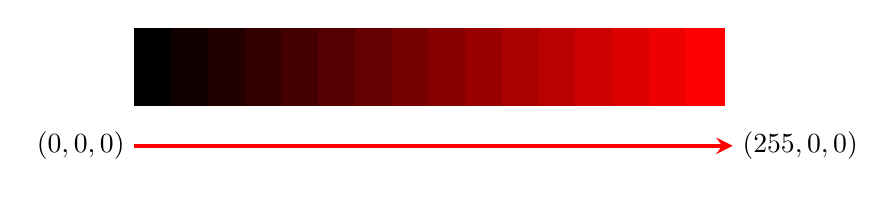
\begin{tikzpicture}
    \foreach \i in {0,17,...,255} {
        \definecolor{rgbred}{RGB}{\i,0,0}
        \fill[fill=rgbred] ({\i/255*7},0) rectangle ++(.5,1);
      }
    \draw[->,ultra thick,draw={rgb:red,1;green,0;blue,0}] (0,-.5) -- (7.6,-.5);
    \node[left] at (0,-.5) {$(0,0,0)$};
    \node[right] at (7.6,-.5) {$(255,0,0)$};
  \end{tikzpicture}
\end{center}

\end{example}


Span of red and blue

\begin{center}
  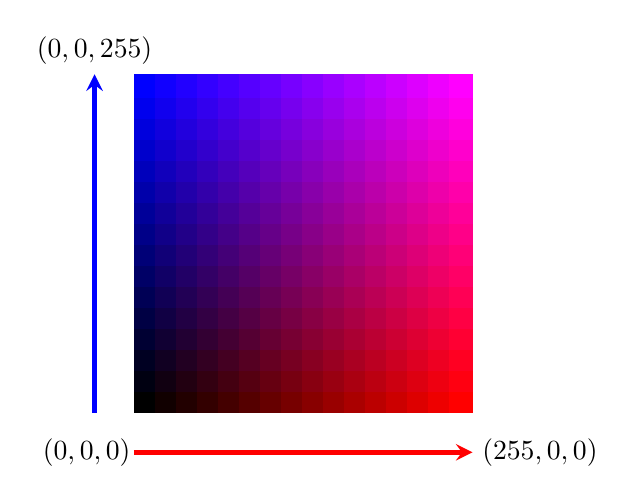
\begin{tikzpicture}
    \foreach \j in {0,17,...,255} {
        \foreach \i in {0,17,...,255} {
            \definecolor{rgbcolor}{RGB}{\i,0,\j}
            \fill[fill=rgbcolor] ({\i/255*4},{\j/255*4}) rectangle ++(.3,.3);
          }}
    \draw[->,ultra thick,draw={rgb:red,1;green,0;blue,0}] (0,-.5) -- (4.3,-.5);
    \draw[->,ultra thick,draw={rgb:red,0;green,0;blue,1}] (-.5,0) --
    (-.5,4.3);
    \node at (-.6,-.5) {$(0,0,0)$};
    \node[right] at (4.3,-.5) {$(255,0,0)$};
    \node[above] at (-.5,4.3) {$(0,0,255)$};
  \end{tikzpicture}
\end{center}

Span of red and green

\begin{center}
  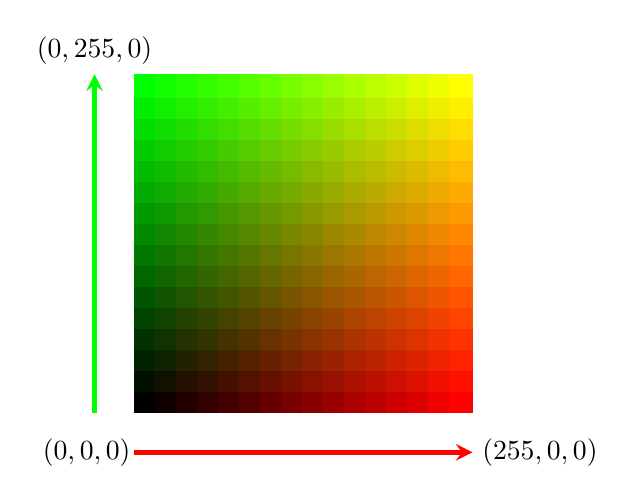
\begin{tikzpicture}[scale=1]
    \foreach \j in {0,17,...,255} {
        \foreach \i in {0,17,...,255} {
            \definecolor{rgbcolor}{RGB}{\i,\j,0}
            \fill[fill=rgbcolor] ({\i/255*4},{\j/255*4}) rectangle ++(.3,.3);
          }}
    \draw[->,ultra thick,draw={rgb:red,1;green,0;blue,0}] (0,-.5) -- (4.3,-.5);
    \draw[->,ultra thick,draw={rgb:red,0;green,1;blue,0}] (-.5,0) -- (-.5,4.3);
    \node at (-.6,-.5) {$(0,0,0)$};
    \node[right] at (4.3,-.5) {$(255,0,0)$};
    \node[above] at (-.5,4.3) {$(0,255,0)$};
  \end{tikzpicture}
\end{center}

Span of blue and green

\begin{center}
  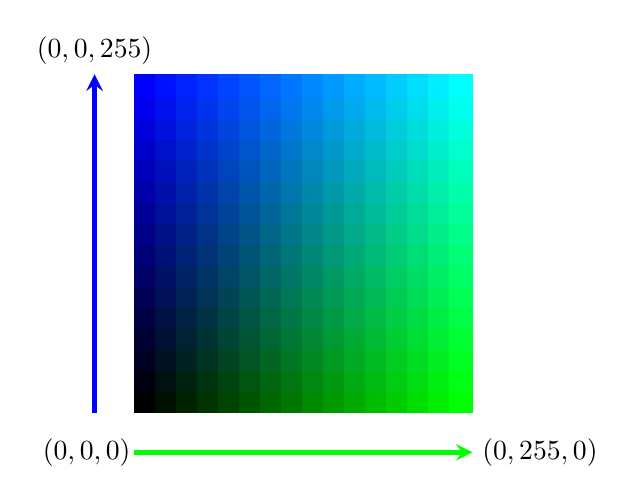
\begin{tikzpicture}
    \foreach \j in {0,17,...,255} {
        \foreach \i in {0,17,...,255} {
            \definecolor{rgbcolor}{RGB}{0,\i,\j}
            \fill[fill=rgbcolor] ({\i/255*4},{\j/255*4}) rectangle +(.3,.3);
          }}
    \draw[->,ultra thick,draw={rgb:red,0;green,1;blue,0}] (0,-.5) -- (4.3,-.5);
    \draw[->,ultra thick,draw={rgb:red,0;green,0;blue,1}] (-.5,0) -- (-.5,4.3);
    \node at (-.6,-.5) {$(0,0,0)$};
    \node[right] at (4.3,-.5) {$(0,255,0)$};
    \node[above] at (-.5,4.3) {$(0,0,255)$};
  \end{tikzpicture}
\end{center}

\begin{definition}
  Given a set of vectors $S$, in a $K$-vector space, $V$, the
  \dfn{span} of the vectors in $S$ is
  \[
    \Span(S) = \left\{\sum_{i=1}^n a_i\sigma_i:\text{$n\in \N$,
      $\sigma_i\in S$, and $a_i\in K$}\right\}.
  \]
  If $\Span(S) = V$, then we say $S$ is a \dfn{spanning set}.
\end{definition}

\subsection{Linear indendence of vectors}

Red is independent from blue in green, as red is not in the span of blue and
green:

\begin{center}
  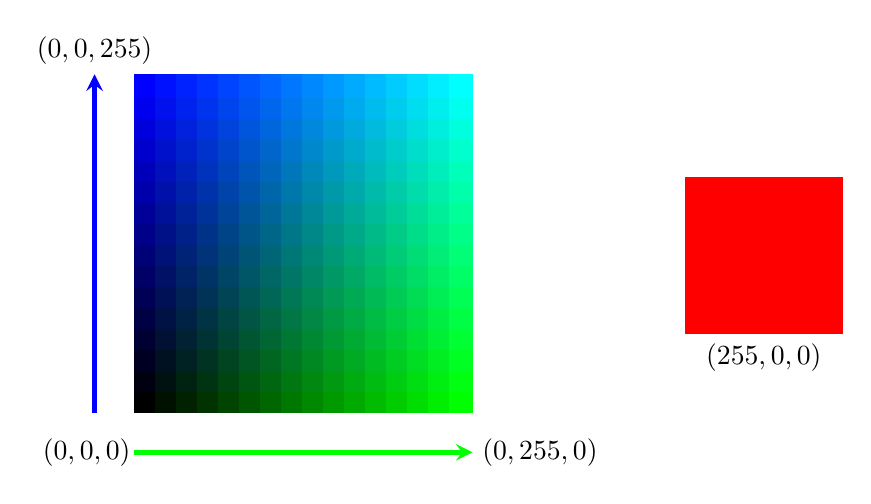
\begin{tikzpicture}
    \foreach \j in {0,17,...,255} {
        \foreach \i in {0,17,...,255} {
            \definecolor{rgbcolor}{RGB}{0,\i,\j}
            \fill[fill=rgbcolor] ({\i/255*4},{\j/255*4}) rectangle +(.3,.3);
          }}
    \draw[->,ultra thick,draw={rgb:red,0;green,1;blue,0}] (0,-.5) -- (4.3,-.5);
    \draw[->,ultra thick,draw={rgb:red,0;green,0;blue,1}] (-.5,0) -- (-.5,4.3);
    \node at (-.6,-.5) {$(0,0,0)$};
    \node[right] at (4.3,-.5) {$(0,255,0)$};
    \node[above] at (-.5,4.3) {$(0,0,255)$};
    \fill[fill={rgb:red,1;green,0;blue,0}] (7,1) rectangle (9,3);
    \node[below] at (8,1) {$(255,0,0)$};
  \end{tikzpicture}
\end{center}

On the other hand, this color is not independent from blue and green as it is
in the span.
\begin{center}
  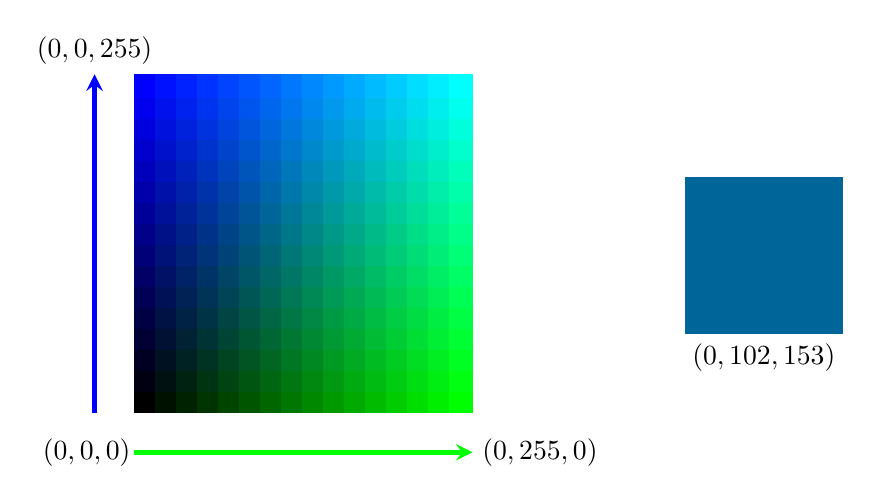
\begin{tikzpicture}
    \foreach \j in {0,17,...,255} {
        \foreach \i in {0,17,...,255} {
            \definecolor{rgbcolor}{RGB}{0,\i,\j}
            \fill[fill=rgbcolor] ({\i/255*4},{\j/255*4}) rectangle +(.3,.3);
          }}
    \draw[->,ultra thick,draw={rgb:red,0;green,1;blue,0}] (0,-.5) -- (4.3,-.5);
    \draw[->,ultra thick,draw={rgb:red,0;green,0;blue,1}] (-.5,0) -- (-.5,4.3);
    \node at (-.6,-.5) {$(0,0,0)$};
    \node[right] at (4.3,-.5) {$(0,255,0)$};
    \node[above] at (-.5,4.3) {$(0,0,255)$};
    \fill[fill={rgb:red,0;green,.4;blue,.6}] (7,1) rectangle (9,3);
    \node[below] at (8,1) {$(0,102,153)$};
  \end{tikzpicture}
\end{center}

Getting somewhere
\begin{center}
  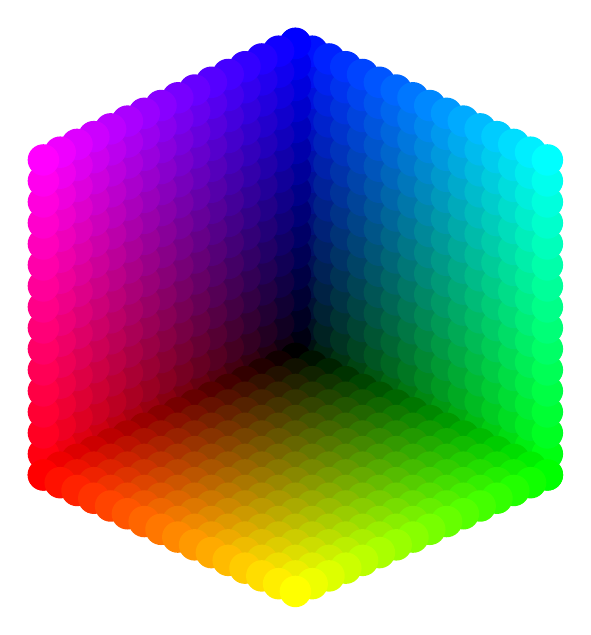
\begin{tikzpicture}
    \foreach \k in {0,17,...,255} {
        \foreach \j in {0,17,...,255} {
            \definecolor{rgbcolor}{RGB}{0,\j,\k}
            \fill[fill=rgbcolor] ({\j/255*4*(.8)},{\k/255*4+(\j)/255*4*(-.37)})
            circle (.2);
          }}
    \foreach \k in {0,17,...,255} {
        \foreach \i in {0,17,...,255} {
            \definecolor{rgbcolor}{RGB}{\i,0,\k}
            \fill[fill=rgbcolor]
            ({\i/255*4*(-.8)},{\k/255*4+(\i)/255*4*(-.37)})
            circle (.2);
          }}
    \foreach \j in {0,17,...,255} {
        \foreach \i in {0,17,...,255} {
            \definecolor{rgbcolor}{RGB}{\i,\j,0}
            \fill[fill=rgbcolor]
            ({\i/255*4*(-.8)+\j/255*4*(.8)},{(\i+\j)/255*4*(-.37)}) circle
            (.2);
          }}
  \end{tikzpicture}
\end{center}

\begin{definition}
  Given a $K$-vector space $V$, a finite set of vectors
  \[
    \{\lambda_1,\dots,\lambda_n\}
  \]
  is said to be \dfn{linearly independent} if
  \[
    a_1\lambda_1 + a_2\lambda_2 +\cdots + a_n\lambda_n = 0\quad \Rightarrow
    \quad
    a_1= \cdots =a_n = 0.
  \]
  A finite set of vectors is set to be \dfn{linearly dependent} if
  they are not linearly independent.
\end{definition}


\section{Four fundamental vector spaces}


\begin{definition}\index{K-vector space@$K$-vector space}\index{vector
  space@$K$-vector space}
A \textbf{$\boldsymbol{K}$-vector space} is an Abelian group $(V,+)$
with identity $\vec{0}$, along with a field $K$ such that we may
multiply group elements by field elements, meaning that there is a
binary operation $-\cdot-: K\times V \to V$ such that if $\nu,\mu\in
  V$ and $a,b,\in K$ we have:
\begin{description}
  \item[Compatibility with scalars] $(ab)\cdot \nu = a\cdot (b\cdot \nu)$.
  \item[Vectors distribute over scalars] $(a+b)\cdot \nu =
      a\cdot\nu + b\cdot \nu$.
  \item[Scalars distribute over vectors] $a\cdot (\nu+\mu) =
      a\cdot \nu + a\cdot \mu$.
  \item[Identity is respected] $1_K\cdot \nu = \nu$.
\end{description}
In this case, elements of the group $V$ are called \dfn{vectors} and
elements of the field $K$ are called \dfn{scalars}.
\end{definition}

\begin{lemma}[Subspace criterion]\index{subspace criterion}
Let $V$ be a $K$-vector space. $W\subset V$ is a subspace of $V$ if
and only if
\begin{enumerate}
  \item $W\ne \emptyset$.
  \item $W$ is closed under multiplication by scalars.
  \item $W$ is closed under vector addition.
\end{enumerate}
\end{lemma}

Here is a picture that attempts to convey the situation:
\[
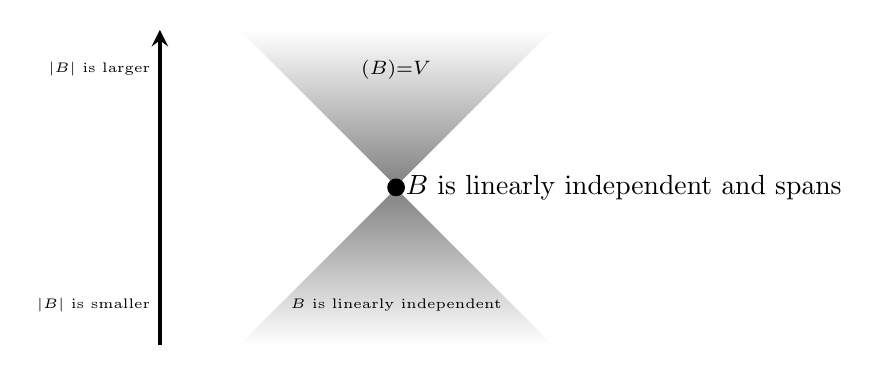
\begin{tikzpicture}
  \draw[white,thin,shading = axis, top color = white, bottom color = gray] (-2,2) -- (0,0)-- (2,2) -- (-2,2) -- cycle;
  \draw[white,thin,shading = axis, bottom color = white, top color = gray] (-2,-2) -- (0,0)-- (2,-2) -- (-2,-2) -- cycle;
  \filldraw (0,0) circle (3pt);
  \node[right] at (0,0) {$B$ is linearly independent and spans};
  \node at (0,1.5) {$\scriptstyle \Span(B) = V$};
  \node at (0,-1.5) {\tiny $B$  is linearly independent};
  \draw[->,ultra thick] (-3,-2) -- (-3,2);
  \node[left] at (-3,-1.5) {\text{\tiny $|B|$ is smaller}};
  \node[left] at (-3,1.5) {\text{\tiny $|B|$ is larger}};
\end{tikzpicture}
\]
The cone above $B$ are all sets of vectors that span $V$. The cone
below $B$ are all sets of vectors that are linearly independent.

\end{document}
